\documentclass[tikz,border=8pt]{standalone}
% Shared look for every TikZ diagram. Load with \input{../../tools/tikz-style.tex}
\usepackage[sfdefault]{roboto}
\usetikzlibrary{arrows.meta, positioning, shapes.geometric, calc, fit, backgrounds}
\definecolor{cblue}{HTML}{4C78A8}
\definecolor{corange}{HTML}{F58518}
\definecolor{cgreen}{HTML}{54A24B}
\definecolor{cred}{HTML}{E45756}
\definecolor{cpurple}{HTML}{B279A2}
\definecolor{cgrey}{HTML}{6B6B6B}
\tikzset{
  every picture/.style={font=\sffamily, line width=1.2pt},
  box/.style={draw=#1, fill=#1!12, rounded corners=4pt, align=center, inner sep=7pt, minimum height=1.1cm},
  box/.default=cgrey,
  arrow/.style={-{Stealth[length=3mm]}, draw=cgrey, line width=1.4pt},
  title/.style={font=\sffamily\bfseries\Large},
  note/.style={font=\sffamily\small, text=cgrey, align=center},
}
\AtBeginDocument{\hyphenpenalty=10000 \exhyphenpenalty=10000}

% The planning levels (Paden et al. 2016, Fig. II.1), with this Note's room on the right: the global plan is made
% once from the map; the local planner re-plans the next 1.5 m every 0.1 s (the rate and window of the ROS benchmark
% in Roesmann et al. 2021: global plan every 2 s, local planner at 10 Hz, 1.5 m of plan).
\begin{document}
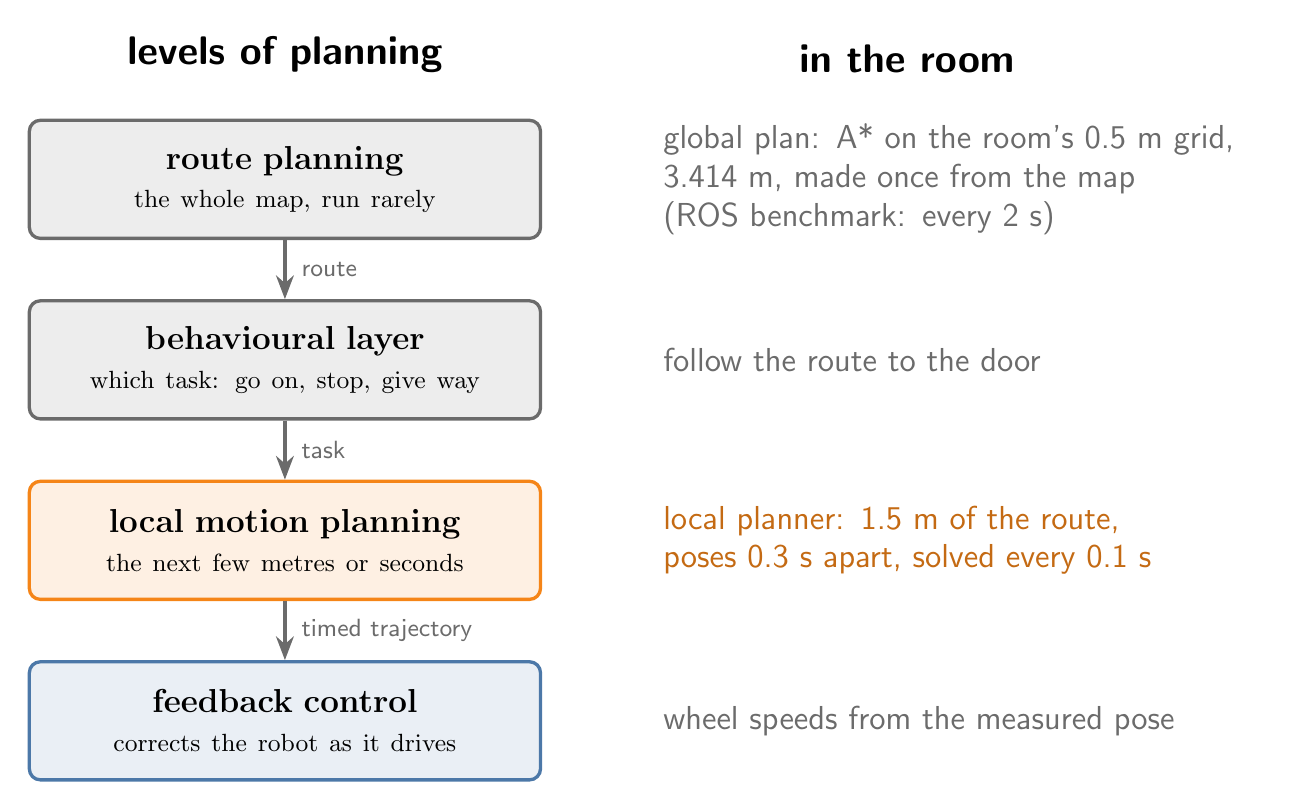
\begin{tikzpicture}[every node/.append style={font=\large}, node distance=0.75cm,
  lv/.style={box=#1, minimum width=6.4cm, text width=6.0cm, minimum height=1.5cm},
  ex/.style={note, font=\sffamily\large, text width=7.6cm, align=left, anchor=west}]
  \node[lv=cgrey] (r) {\textbf{route planning}\\ \small the whole map, run rarely};
  \node[lv=cgrey, below=of r] (b) {\textbf{behavioural layer}\\ \small which task: go on, stop, give way};
  \node[lv=corange, below=of b] (m) {\textbf{local motion planning}\\ \small the next few metres or seconds};
  \node[lv=cblue, below=of m] (c) {\textbf{feedback control}\\ \small corrects the robot as it drives};
  \draw[arrow] (r) -- node[note, right, xshift=2pt] {route} (b);
  \draw[arrow] (b) -- node[note, right, xshift=2pt] {task} (m);
  \draw[arrow] (m) -- node[note, right, xshift=2pt] {timed trajectory} (c);
  \node[ex, right=1.4cm of r] {global plan: A* on the room's 0.5 m grid,\\ 3.414 m, made once from the map\\ (ROS benchmark: every 2 s)};
  \node[ex, right=1.4cm of b] {follow the route to the door};
  \node[ex, right=1.4cm of m, text=corange!80!black] {local planner: 1.5 m of the route,\\ poses 0.3 s apart, solved every 0.1 s};
  \node[ex, right=1.4cm of c] {wheel speeds from the measured pose};
  \node[title, above=0.45cm of r] {levels of planning};
  \node[title, above=0.45cm of r, xshift=7.9cm] {in the room};
\end{tikzpicture}
\end{document}
